\chapter{Evaluation}

In this paper we have also empirically evaluated how effective deadlock exception can be.

We had two implementations of reentrant locks where one of them was the one provided by
Java's \emph{ReentrantLock} and the other was that lock modified to throw exception when
a deadlock happened. Later we may refer to our implementation as \emph{LockA} and the default
one as \emph{LockB}.

In order to compare each implementation, we conducted
a controlled experiment where students had to run two specific programs with deadlocks
easy to reproduce while collecting the time taken to identify the problem. They also
had to provide a clear explanation of the problem, describing what the problem is, which method
calls were involved on it and a description of how it happens, so we could measure answer precision.

\section{Experiment Definition}

The goal of our experiment was to analyze the process of bug identification with the purpose of evaluating efficiency of deadlock exceptions,
in respect to the time spent in order to identify the problem and the accuracy of the descriptions provided by the students. We can define two
research questions we want to answer in this experiment:

{\bf RQ1.} Is the time spent to identify the bug reduced for implementation with deadlock exception when compared to the default implementation?

The metric we watched to answer this question was the time, in seconds, to finish each question in the test.

{\bf RQ2.} Is the accuracy of bug description improved for implementation with deadlock exception when compared to the default one?

Each question's answer was splitted in a few criterias and each criteria was rated between 0 and 1, where 0 means not present, 0.5 means partially present and 1 for fully present:

\begin{description}
\item[A.] Correctly classified problem as deadlock.
\item[B.] Classified problem as different from deadlock.
\item[C.] Correctly identified method calls involved in the deadlock.
\item[D.] Correctly identified locks involved in the deadlock. 
\item[E.] Pointed unrelated methods as part of the deadlock.
\end{description}

To answer this research question, we have classified students answers as either correct or incorrect. Correct answers should respect the following equation:

\begin{equation}
  (A - B) + C \geq 1.5 \;
\end{equation}

We decided to rule out criterias \emph{D} and \emph{E} because the problem statement was not clear they should describe which locks were involved in the deadlock; also, our deadlock implementation at that time could only guarantee at least one deadlock exception to be thrown thus affecting at least one method. In other words, this equation means that a correct answer is whenever the bug was described as deadlock and at least one of the methods involved were identified.

\section{Experiment Planning}

In order to evaluate each element described on the previous section, we describe the following statistical hypotheses.

\subsection{Hypothesis}

To answer \emph{RQ1} regarding the time spent to identify a bug in the code:

\begin{equation}
  H_{0} : \mu_{TimeLockA} \geq \mu_{TimeLockB}
\end{equation}
\begin{equation}
  H_{1} : \mu_{TimeLockA} < \mu_{TimeLockB}
\end{equation}

And to answer \emph{RQ2} regarding accuracy of answers:

\begin{equation}
  H_{0} : \mu_{CorrectAnswersLockA} \leq \mu_{CorrectAnswersLockB}
\end{equation}
\begin{equation}
  H_{1} : \mu_{CorrectAnswersLockA} > \mu_{CorrectAnswersLockB}
\end{equation}

\subsection{Design, Instrumentation and Subjects}

For this empirical experiment, we have chosen two metrics: time to answer a question and number of correct answers.

In order to prevent \emph{bias}, we needed to control a few factors during the experiment execution. The first factor was the selection of subjects to participate on this experiment, as different background knowledge could potentially influence chosen metrics. The second factor we had to control was the complexity of programs that each subject. Complexity we define as the amount of files in the program, number of threads and number of locks to analyze; as we've assumed that easier programs could have little or no benefit from deadlock exceptions, we wanted to have one program that we considered easy to identify the problem and another that was more complex and composed by many files and classes, reflecting a more realistic case. We provided implementations of each program using either \emph{LockA} or \emph{LockB}: the two possible treatments that we want to compare.

We decided to use Latin Square Design to control these two factors mentioned earlier: subjects and program complexity factors. Since we had N subjects, 2 programs and 2 possible treatments, we disposed subjects in rows and programs in columns of latin squares, randomly assigning in each cell of the square a treatment that could be \emph{LockA} or \emph{LockB}, but also guaranteeing that for any given row or column in this square, each treatment appears only once (see Table 1). Consequently, we have replication, local control and randomization which are the three principles of experiment design \cite{box}.

\begin{table}
\begin{center}
\caption{Latin Square design}
\begin{tabular}{|l|l|l|}
\hline
 & Program 1 & Program 2\\
\hline
Subject 1 & LockA & LockB\\
Subject 2 & LockB & LockA\\
\hline
\end{tabular}
\end{center}
\end{table}

We wrote two programs with different complexity which were presented in the same order for all subjects. The first program, known as \emph{Bank}, contained 4 classes spread in 4 files, 3 threads, 3 explicit locks, and 82 lines of code in average. The second program, known as \emph{Eclipse} had 15 classes spread in 11 files, 4 threads, 5 explicit locks, and 40 lines of code in average. We expected the first program to be easier to identify the deadlock because it contained fewer classes and files. Each program could use either \emph{LockA} or \emph{LockB} but we randomly assigned a group to each student so that if they fall into group A, they would start with \emph{LockA} in the first question, but change to \emph{LockB} on the second question; or if they fall in group B, they they would start with \emph{LockB} and switch to \emph{LockA} in the second question. We randomly paired subjects in tuples composed of one subject in group A and another subject of group B, then we created latin squares for each one of these pairs, where any remainders were discarded.

% insert each program description here, where the deadlock was, etc. in the end, point to where the source for each pdf is %

We have repeated this experiment for two groups of students with different backgrounds. The first group consisted of undergraduate students attending Programming Language Paradigms course. They had classes about concurrent programming, including exercises in Java using ReentrantLock where deadlocks and other concurrent bugs should be avoided; however, these students were not experienced in this area. The second group consisted of graduate students enrolled in master's degree or PhD program attending Parallel Programming course where they had classes about advanced concepts of parallel programming and had a lot of practical exercises, including implementing their own lock; thus, they were expected to have a lot of experience. We did a survey with the second group to understand their background even further (see charts below) at the end of the experiment.

% TODO: insert chart with survey results

\subsection{Metrics Collection}

Each one should start the experiment with the first question containing \emph{Program 1} and once they finish to provide an answer, they should request for the second question. At that point, we collect and place a timestamp in their answer. Once they finish the second question containing \emph{Program 2}, then they should again give us a notice so we can leave a new timestamp. We have used these timestamps to measure how long they took to finish each question. We have started this experiment with a time limit for each question of 60 minutes each. However, during the test we realized it could not be sufficient for all students so we expanded to 90 minutes each.

The timestamp was written by students conducting the experiment based on a counter we projected on the laboratory wall in real time. In a few circunstances the subject could write the timestamp when they finish, but we have double checked the value at the time we collected their answer, overwriting in case they did any mistake.

\section{Experiment Operation}

We executed this experiment in two different days. In the first day we did it with undergraduate students in replacement of their default exam, so their participation was obligatory but we disclaimed they could optionally leave a comment if they did not want to take part in this research, so we would not use their data. Fortunately no one chose to not participate. In the second day, we did it with graduate students after the last class of Parallel Programming course and it was optional. In total, 31 students participated on the first day and 16 students participated on the second day, but we had to discard 2 students data because they arrived late and they had to leave early.

On the first day we started with a time frame of 2 hours for the whole experiment, so we decided to set a deadline for each question and put a time limit of 1 hour each. Later we expanded the time limit to 1 hour 30 minutes for each question. On the second day we decided to stick with 1 hour each because there was no demand to extend it.

\section{Experiment Results}

We can split the experiment analysis in two parts: time and accuracy.

\subsection{Time Analysis}

Time analysis was conducted with R Statistical Software using the inputs\footnote{We provide the inputs we've used in the appendix.} extracted from each experimentation day. We've used the linear model described in Figure 1 that considers the effect of different factors on the response variable similarly to Paola's work \cite{paola}, but we've also added the effect between each replica and the treatment as explained by Sanchez in \cite{sanchez}.

\begin{figure}
\begin{center}
$Y_{lijk} = \mu + \tau_{l} + \tau\alpha_{li} + \beta_{j} + \gamma_{k} + \tau\gamma_{lk} + \epsilon_{lijk}$\\
\vspace{4mm}
\begin{tabular}{ll}
$Y_{lijk}$ & - response of $l_{th}$ replica, $i_{th}$ student, $j_{th}$ program, $k_{th}$ lock \\
$\tau_{l}$ & - effect of $l_{th}$ replica \\
$\tau\alpha_{li}$ & - effect of interaction between $l_{th}$ replica and $i_{th}$ student \\
$\beta_{j}$ & - effect of $j_{th}$ program \\
$\gamma_{k}$ & - effect of $k_{th}$ lock \\
$\tau\gamma_{lk}$ & - effect of interaction between $l_{th}$ replica and $k_{th}$ lock \\
$\epsilon_{lijk}$ & - random error \\
\end{tabular}
\caption{Regression model.}
\end{center}
\end{figure}

Initially, we've plotted the box-plot graphic shown in Figure 2. We can see that answers with \emph{LockB} involved took more time to complete, but suddenly stop to grow not far from where \emph{LockA} reaches its peak. If there was no time limit on each question, we believe that \emph{LockB} times would show a much wider range.

\begin{figure}
\centering
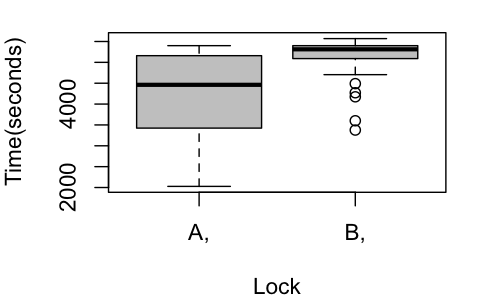
\includegraphics[height=4.5cm]{img/u1.png}
\caption{First experiment box-plot graphic.}
\end{figure}

Then we've run the Box-Cox transformation - which is a power transformation - to reduce anomalies such as non-addivity and non-normality, obtaining the curve in the left of Figure 3. Since the value of $\lambda$ at the maximum point in the curve is not approximately 1, we should apply the transformation; that is, $Y_{lijk}$ should be powered to that $\lambda$ on our regression model. Running the same analysis again with the transformed model, we obtain the curve shown in the right of Figure 3.

\begin{figure}
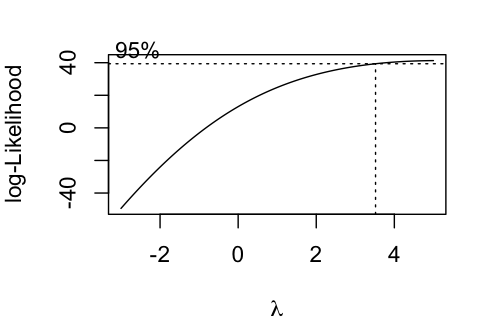
\includegraphics[height=4.5cm, width=6cm]{img/u2.png}
\hfill
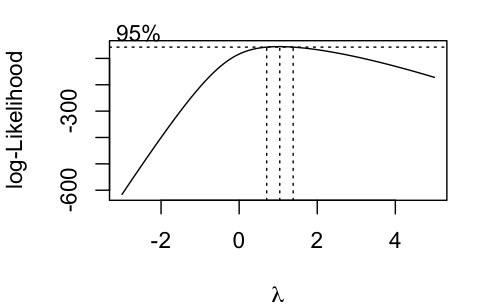
\includegraphics[height=4.3cm, width=6cm]{img/u2boxcox.png}
\caption{First experiment: before and after box-cox transformation ($\lambda = 5$).}
\end{figure}
\\

After applying Box-Cox transformation, we ran Tukey Test of Additivity that checks whether effect model is additive, so we can evaluate whether interaction between factors displayed on the rows and columns of each latin square won't affect significantly the response when the model is additive \cite{box}; thus, considering the following hypothesis:

\begin{tabular}{ll}
$H_{0}$ & : The model is additive \\
$H_{1}$ & : $H_{0}$ is $false$ \\
\end{tabular}

We have obtained a p-value of 0.514, which means we cannot reject $H_{0}$. Consequently the model was considered to be additive.

Finally, we ran the ANOVA (ANalysis Of VAriance) test which compares the effect of treatments on the response variable, providing an approximated p-value for every associated factor. When a variable has \emph{p-value} $< 0.05$, it means that factor was significant to the response.

\begin{table}
\begin{center}
\caption{Undergraduate students experiment ANOVA results.}
\begin{tabular}{|l|l|l|l|l|ll|}
\hline
                & Df &    Sum Sq  &  Mean Sq   & F value & \emph{p-value} &     \\  
Replica         & 14 & 3.8633e+37 & 2.7595e+36 & 1.6553  & 0.1784197 &     \\   
Program         & 1  & 4.1460e+36 & 4.1460e+36 & 2.4869  & 0.1371197 &     \\   
Lock            & 1  & 3.9489e+37 & 3.9489e+37 & 23.6873 & 0.0002492 & *** \\
Replica:Student & 15 & 4.1013e+37 & 2.7342e+36 & 1.6401  & 0.1808595 &     \\  
Replica:Lock    & 14 & 2.4033e+37 & 1.7166e+36 & 1.0297  & 0.4785520 &     \\  
Residuals       & 14 & 2.3340e+37 & 1.6671e+36 &         &           &     \\
\hline
\end{tabular}
\end{center}
\end{table}

In Table 4, we can see that \emph{Lock} factor was the most significant to the response, allowing us to reject our null hypothesis defined in Equation 10.

Now we will show the results collected by the second experiment with graduate students. They were exposed to the same set of problems in a different day, but as explained before, they only had a time limit of 1 hour per question.

When we analyze the box-plot for the second group displayed in Image, we can see there was a clear improvement on the time for students with \emph{LockA}.

\begin{figure}
\centering
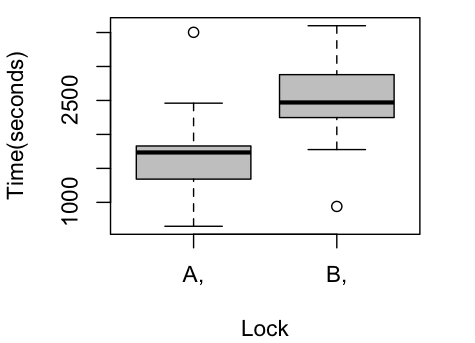
\includegraphics[height=4.5cm]{img/g1.png}
\caption{Second experiment box-plot graphic.}
\end{figure}

Moving foward with the analysis, we check if a box-cox transformation is needed. Since the value is not approximately 1, we apply the power transformation the same way we did with the first experiment, but with the corresponding lambda value.

\begin{figure}
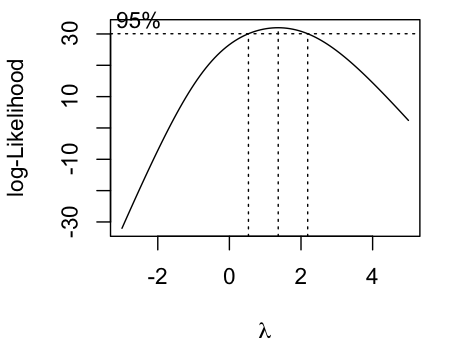
\includegraphics[height=4.5cm]{img/g2.png}
\hfill
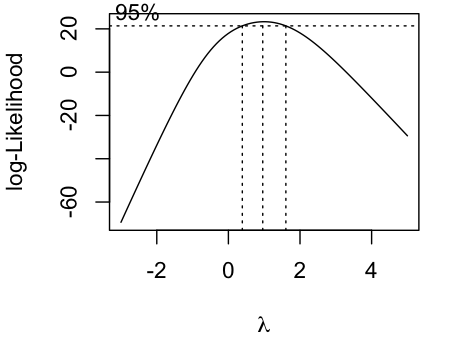
\includegraphics[height=4.4cm]{img/g2boxcox.png}
\caption{Before and after box-cox transformation ($\lambda = 1.3636$).}
\end{figure}

Finally, running ANOVA, we can see that the type of lock was the most significant factor for the response time, as shown in Table 3. Again, we can reject the null hypothesis.

\begin{table}
\begin{center}
\caption{Graduate students ANOVA results.}
\begin{tabular}{|l|l|l|l|l|ll|}
\hline
                 & Df &    Sum Sq &   Mean Sq  & F value &   Pr(>F) & \\   
\hline
replica          & 6 & 2576883250 &  429480542 & 14.1891 & 0.0025793 & **  \\
program          & 1 &    6875586 &    6875586 &  0.2272 & 0.6505035 &     \\
lock             & 1 & 1958179433 & 1958179433 & 64.6938 & 0.0001975 & *** \\
replica:student  & 7 & 2328154077 &  332593440 & 10.9881 & 0.0047601 & **  \\
replica:lock     & 6 &  823830276 &  137305046 &  4.5362 & 0.0441188 & *   \\
Residuals        & 6 &  181610625 &   30268438 &         &           &     \\
\hline
\end{tabular}
\end{center}
\end{table}

In the end of this paper, we provide the list of inputs and instructions on how to reproduce these results as attachments.

\subsection{Accuracy Analysis}

Once we collected all answers, we manually evaluated each one of them according to the criterias established previously, where each criteria had an associated value between 0 and 1. Then we've ran a script that evaluates the equation we defined before to classify whether an answer was correct or not. Grouping the results in tables, we have Table 4 and Table 5.

\begin{table}
\begin{center}
\caption{Undergraduate students answers accuracy}
\begin{tabular}{|l|l|l|}
\hline
 & Correct & Incorrect\\
\hline
LockA & 29 & 2\\
LockB & 16 & 15\\
\hline
\end{tabular}
\end{center}
\end{table}

\begin{table}
\begin{center}
\caption{Graduate students answers accuracy}
\begin{tabular}{|l|l|l|}
\hline
 & Correct & Incorrect\\
\hline
LockA & 13 & 1\\
LockB & 10 & 4\\
\hline
\end{tabular}
\end{center}
\end{table}

Applying Fisher's exact test we can see that undergraduate students results presented a two-tailed P value equals 0.0004: the association between rows (groups) and columns (outcomes) is considered to be extremely statistically significant; consequently, there is clear evidence of improvement on accuracy (see Table 4).

Meanwhile graduate students results presented a two-tailed P value equals 0.3259, which does not represent a statistically significant evidence of improvement in accuracy (see Table 5).

The input and the script to generate the tables are available as attachments in the end of this paper.

% TODO: add script and the data used (anonymized) to appendices or put on github and link %

\section{Discussion}

% TODO: review this section, it was written based on older results %

We can see in our results that both groups of students have improved their time to solve the problem when they had the lock with deadlock exception. Also, on the first group, we have found statistically significant evidence that it improved answers accuracy, but not for the second group.

We cannot draw conclusions regarding the improved accuracy on the second group, but we can bring up some relevant aspects we've observed and make a few hypothesis. Some students in the second group were greatly experienced on concurrent programming and they knew how to efficiently find a deadlock using the tools available in Eclipse. Thus, they have finished the exercise really quickly for both problems, knowing exactly which points in the code were involved in the deadlock. So we can see that deadlock exceptions are more helpful for unexperienced programmers in general, and it's possible that even if we had a bigger sample for the second group, we would still not see a significant difference that would indicate deadlock exceptions improved their accuracy.

However, we believe that the benefits of deadlock exceptions are beyond helping unexperienced programmers to find deadlocks more precisely. Experienced programmers would still benefit in many cases where the deadlock is not as obvious as in the exercise we've presented. For example, in a more realistic situation, a deadlock can happen in a background thread that doesn't really affect the program execution overall but make the execution lacking some expected behavior. Furthermore, in non-interactive systems where they are only running in background, is nearly impossible to know when there's a problem unless this software is monitored constantly which is very time consuming or the system produces output constantly that is affected by a potential deadlock. If we have a deadlock exception, we can either prepare and handle this exception on the code level, or just have this signal from output that would help developers to fix it later.

\section{Threats To Internal Validity}

In this experiment, we've collected evidence on how the presence of deadlock exception affects student ability to identify deadlocks accurately. However, we must raise a few considerations regarding the validity of our results.

\subsection{Time Measurement}

Since we wanted to run the experiment in a homogenous environment, we've decided to run it in a laboratory in Federal University of Pernambuco, and we've provided links to download the exercise and a few instructions explaining how to deploy it. We wanted to make it as easy as possible and before we've started the test, we gave a small presentation reproducing step by step the instructions that would be described on each exercise, so everyone could follow up and make the setup at the same time. Once everyone was done, we've started to count the time and allowed them to run the programs and start debugging. However, this procedure was not enough: there was a few students (approximately 3 in total) who did the setup differently and could not execute the program; therefore, they've lost a few minutes until we've fixed that for them. Since they've lost only a few minutes, we have still counted them as part of the experiment and did not discount the time.

Furthermore, some students arrived at the test more than 10 minutes late. We've allowed them to join, but some of the remaining computers in the laboratory had issues like they were not logging in or the mouse was not working. We've lost a few minutes to make them work or find a new computer and once each of them did the setup, we've started to count their time individually.

Whenever a student finished a given question, if the time was below the time limit they had available, we have marked the current timestamp on each student's name in the whiteboard. Each entry inserted was already sorted by time, so we easily tracked whether each student was close to the second question's time limit. It would have been better to do this automatically rather than doing manually, so we could potentially reduce overhead of these timestamp operations and increase their precision.

Also, we believe that our imposed time limit have limited more drastically the time ranges on the first group because they spent more time on each question. Also the fact it was an exam for them may have delayed the time to answer because they were more careful. We have observed during the experiment that many students wrote their answers but they were reluctant to ask for the next question because they still have plenty of time left and they wanted to make sure it was correct. We did not observe such behavior with the second group of students and we believe it is because they did not have the same pressure to deliver correct results as the first group had.

\subsection{Exercises}

We understand that the two questions we've used to evaluate the students are far easier than what most software engineers have to deal with in the real world. However we could not use any real world issue because it would easily take the time limit of the experiement for each bug.

On the other hand, we've created two questions based on real world bugs that we have found while searching for deadlock bugs in open source repositories. Each question had a particular level of granularity, where one should be easier to find a bug because of the less amount of code to examine and another that should be more difficult because of the reasonable amount of different files to look at.

Some researchers actually believe that empiric evaluations should not be limited to real projects. Buse claims there are benefits of using non-real artifacts \cite{buse} because it's easier for researchers to translate research questions into successful experiments as it allows a greater control over confouding factors. Otherwise, it would be necessary to turn all participants familiar with the codebase of a real and complex system before even starting the experiment. 

\section{Threats to External Validity}

Let's consider a few conditions that might limit the generalization power of our findings in this experiment.

\subsection{Students}

Each student which participated in this experiment had a different background. What we did to minimize the differences was to select groups where students had at least basic experience in concurrent programming and they should be familiarized with the types of bugs such codes can have: the first group of students with undergraduate students attended the class Paradigms of Computaional Languages where deadlocks are covered in classes and exercises; the second group with graduate students attended the class Parallel Programming which covered concurrent programming in low level detail in classes and exercises, including deadlock detection.

Some studies have already addressed the problem of drawing conclusions made with students but some suggest that using students as subjects is as good as using industry professionals \cite{staron}. Runes ran an experiment which shows that there's not much significant differences between undergraduate, graduate and industry professionals, with the exception that undergraduate students often take more time to complete the tasks \cite{runes}.




